\chapter{Results}\label{sec:results}
To verify both the correctness and the gain in terms of speed of execution of the new implementation of the bistable simulation engine many circuits has been simulated both with cpu and gpu.
As already said the parameters that mainly affect simulation time are the number of inputs, which define the samples for the simulation, and the number of cells. We choose a wide range of circuit in order to get a good estimation of the speedup with different designs. We choose circuits with inputs from 2 to 6 and with a minimum of 30 cells to a maximum of 35.000 cells. \newline
In the optimization we focused on parallelization of the computation of cells polarization, so we expected to see lower execution time with respect to the cpu with increasing of the number of cells. This hypothesis has been confirmed by the results of the simulations.

\begin{figure}
\centering
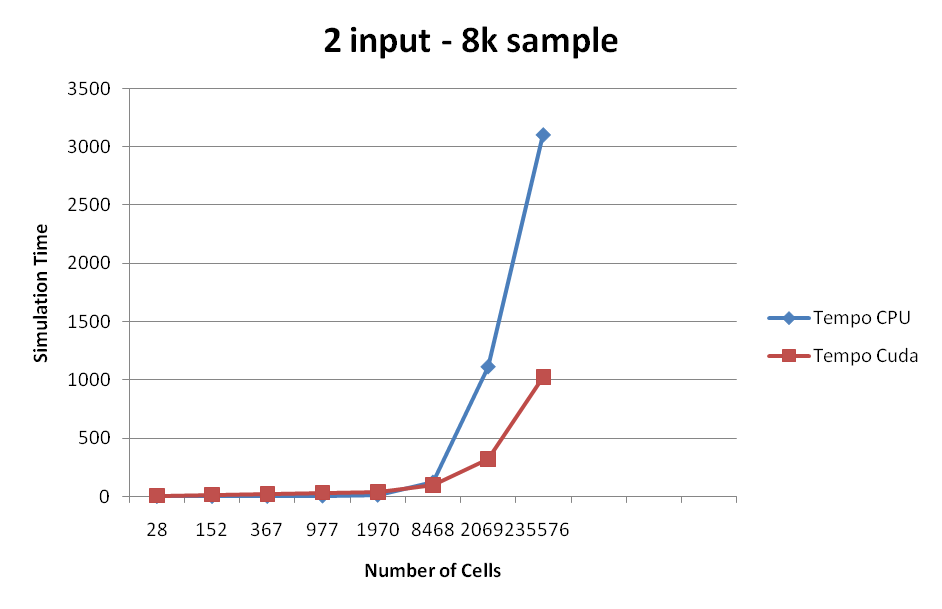
\includegraphics[width=\columnwidth]{img/graph1.png}
\label{graph1}
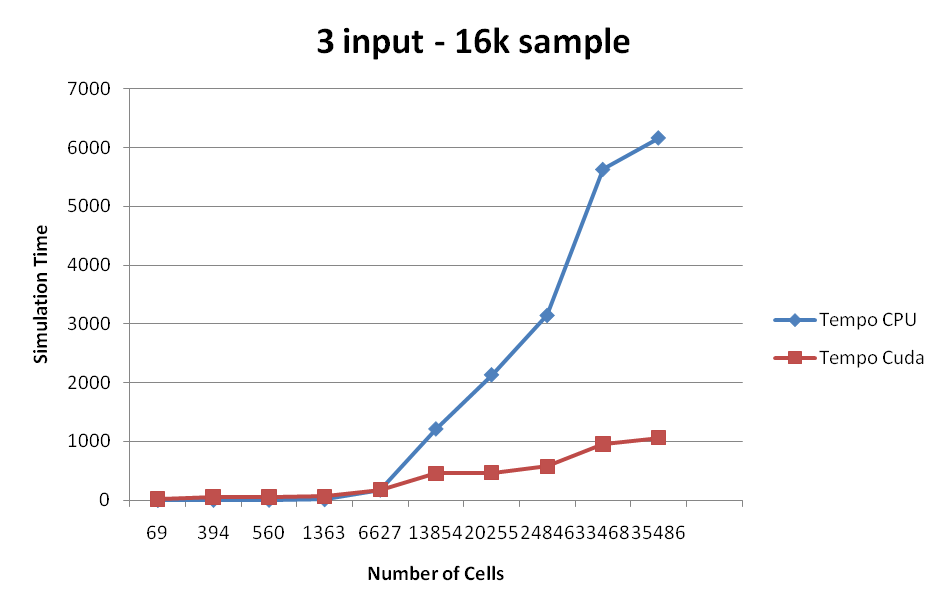
\includegraphics[width=\columnwidth]{img/graph2.png}
\label{graph2}
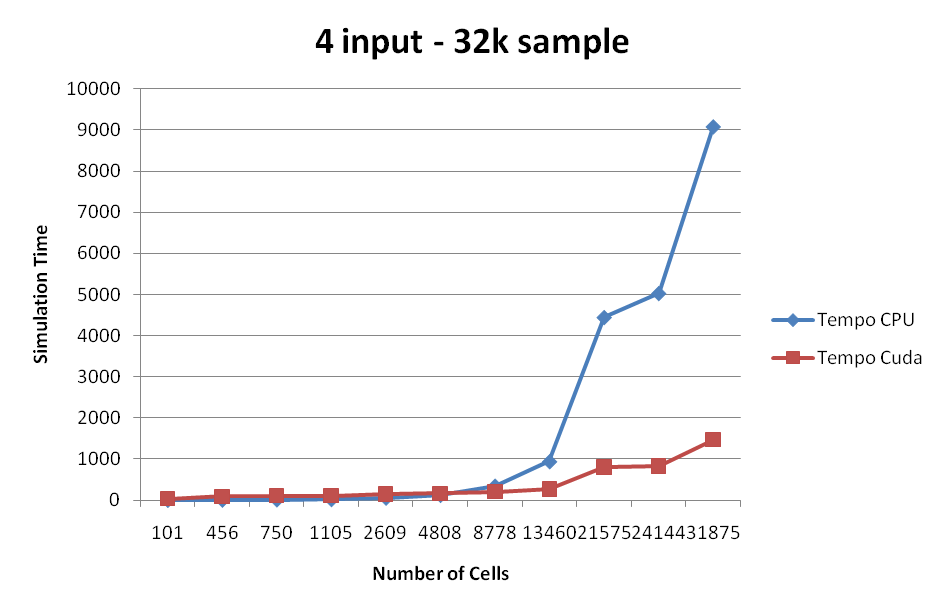
\includegraphics[width=\columnwidth]{img/graph3.png}
\label{graph3}
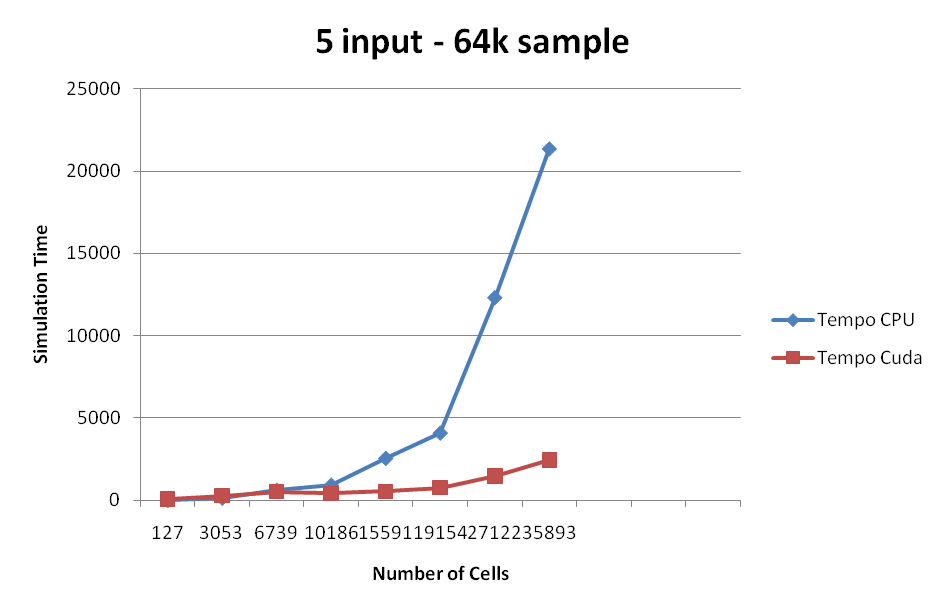
\includegraphics[width=\columnwidth]{img/graph4.png}
\label{graph4}
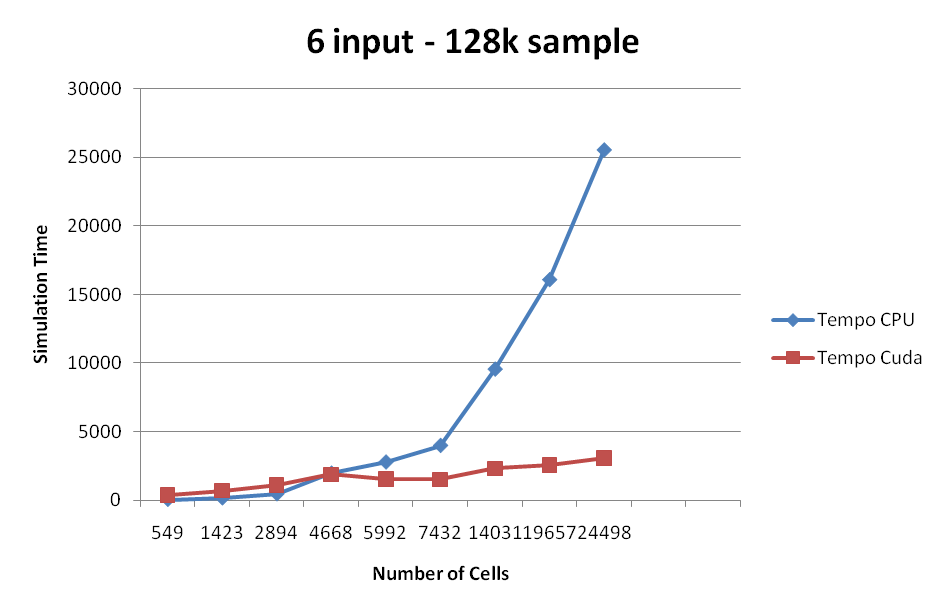
\includegraphics[width=\columnwidth]{img/graph5.png}
\label{graph5}
\includegraphics[width=\columnwidth]{img/graph6.png}
\label{graph6}
\end{figure}